Так как логарифм - обратная функция от показательной, она логично получается поворотом на 90 градусов вправо и также делится на 2 случая, относительно параметра a.

\begin{figure}[h!]
	\centering
	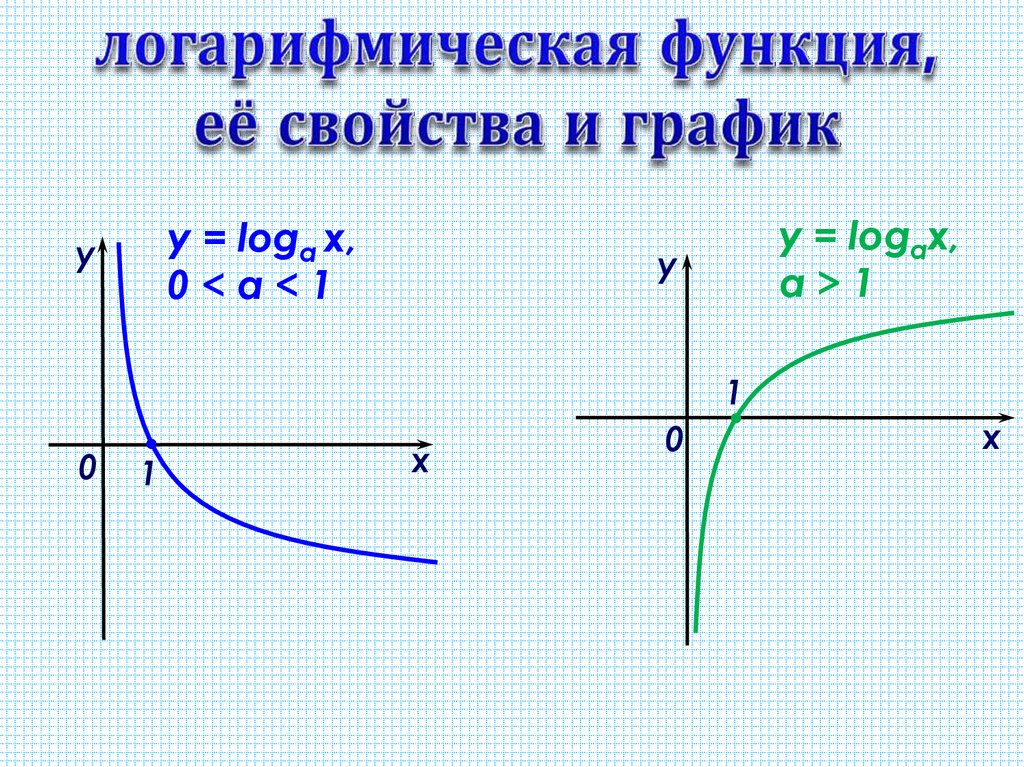
\includegraphics[width=0.6\textwidth]{img/log.jpg}
	\caption{Логарифмическая функция}
\end{figure}